\documentclass[12pt]{article}
\usepackage[utf8]{inputenc}
\usepackage{tikz,egplot}
\usepackage[margin=1in]{geometry}
\usepackage{graphicx,ctable}
\usepackage{longtable}
\usepackage{hyperref,xcolor}
\hypersetup{colorlinks=false, linkbordercolor=red,pdfborderstyle={/S/U/W 1}}
\usepackage[para]{threeparttable}
\usepackage{tgpagella}
\usepackage[utf8]{inputenc}
\usepackage{natbib}
\usepackage{caption}
\usepackage{subcaption}
\usepackage{enumitem}
\usepackage{amsmath}
\usepackage[T1]{fontenc}
\setlength{\parindent}{0em}
\usepackage{forest}
\usepackage{hyperref}
\newcommand{\tab}{\hspace*{3em}}
\hypersetup{
colorlinks = true,
urlcolor = blue,
}
\usepackage{setspace,amsfonts,amssymb,url,booktabs,tabularx,amsmath,amsthm}

\title{Persistence of the China Shock according to ADH (2013) specifications}


\date{December 2022}

\begin{document}

\maketitle

\section*{Data}

We use ACS data from \href{https://usa.ipums.org/usa/}{IPUMS}. We pooled three ACS 1-year samples for each year starting in 2006 and ending in 2020.  ACS 1-year samples for 2001-2004 did not have geographic information, so we omitted these years. For each year, we follow ADH 2013 in their data construction.\footnote{We follow David Dorn's ReadMe file to map the PUMAs to CZ. We used the \textbf{cw\_puma2000\_czone.dta} for ACS before 2012 and \textbf{cw\_puma2010\_czone.dta} for ACS files from 2012 to 2021.} 

\section*{Regression specification}

%Figure \ref{fig:three graphs} shows 

We also follow ADH (2013) regression specification (equation 5) to estimate the two-stage least squares coefficients for the impact of exposure to China on manuf. employment, non-manuf. employment, unemployment, and NILF. These coefficients for each year are shown in Figure \ref{fig:three graphs} below. Four things to note. 

\begin{enumerate}
\item We keep fixed the definition of exposure to China (i.e., we fix the change in USA imports from China for the 2000-2007 period).  
\item The main regression specification in ADH (2013) includes the 1990-2000 period and the 2000-2007 period (with variables computed in decadal changes). We follow the same specification including both 1990-2000 and 2000-$\tau$ periods, where $\tau \in \{ 2006,..., 2020 \}$. Each regression for each year has 1444 observations (722 $\times$ 2 periods). 
\item We use the same controls as in ADH (2013) irrespective of the time-horizon. We take these control variables from the ADH (2013) replication file.
\item The coefficients for 2007 in Figure \ref{fig:three graphs} (for manuf. employment, non-manuf. employment, unemployment, and NILF) exactly match those from Table 5, Panel B, Column 1, 2, 3, and 4 in ADH (2013). 
\end{enumerate}


\begin{figure}  \caption{Imports from China and Employment Status of Working-Age Population within CZs. 2SLS Estimates}\label{fig:three graphs}
     {\centering
     \begin{subfigure}[b]{0.45\textwidth}
         \centering
         \caption{Manuf employment/working-age pop.}
         \includegraphics[width=\textwidth]{results/figures/mfg_decadal_adh13.pdf}
     \end{subfigure}
     \hfill
     \begin{subfigure}[b]{0.45\textwidth}
         \centering
         \caption{Non-manuf. employ./working-age pop.}
         \includegraphics[width=\textwidth]{results/figures/nmfg_decadal_adh13.pdf}
     \end{subfigure}
     \hfill
     \begin{subfigure}[b]{0.45\textwidth}
         \centering
         \caption{Unemployed persons/working-age pop.}
         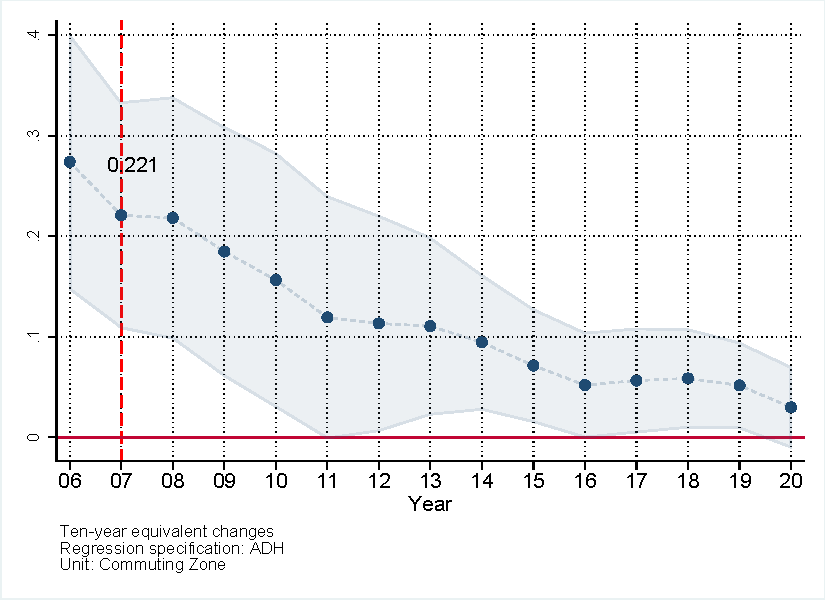
\includegraphics[width=\textwidth]{results/figures/unempl_decadal_adh13.pdf}
     \end{subfigure}
     \hfill
     \begin{subfigure}[b]{0.45\textwidth}
         \centering
         \caption{NILF/working-age pop.}
         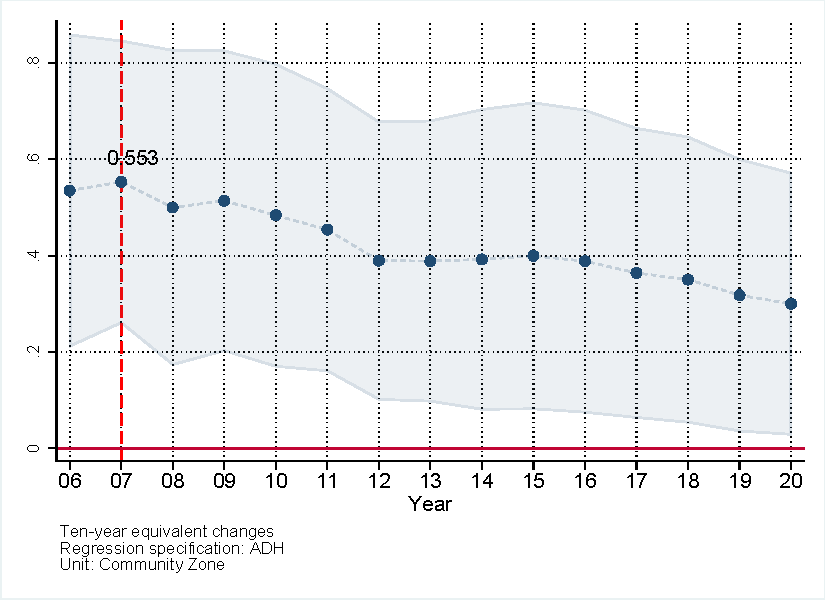
\includegraphics[width=\textwidth]{results/figures/nilf_decadal_adh13.pdf}
     \end{subfigure}}\\
\textit{Note:} Panels report two-stage least squares coefficient estimates and 95 percent confidence intervals for these estimates. The LHS of the regression equation stacks the change in the specified outcome between 1990-2000 and between 2000 and the year indicated on the horizontal axis. The trade shock is the decadalized 2000–2007 change in CZ import exposure, as defined in ADH (2013) and instrumented by the change in import exposure of other countries, as in ADH (2013). Control variables are also the same as in ADH (2013). By construction, the coefficients for 2007 (highlighted with the vertical dashed line) exactly match those from Table 5, Panel B, Column 1, 2, 3, and 4 in ADH (2013).
\end{figure}


\end{document}
